\iffalse
This file is protected by Copyright. Please refer to the COPYRIGHT file
distributed with this source distribution.

This file is part of OpenCPI <http://www.opencpi.org>

OpenCPI is free software: you can redistribute it and/or modify it under the
terms of the GNU Lesser General Public License as published by the Free Software
Foundation, either version 3 of the License, or (at your option) any later
version.

OpenCPI is distributed in the hope that it will be useful, but WITHOUT ANY
WARRANTY; without even the implied warranty of MERCHANTABILITY or FITNESS FOR A
PARTICULAR PURPOSE. See the GNU Lesser General Public License for more details.

You should have received a copy of the GNU Lesser General Public License along
with this program. If not, see <http://www.gnu.org/licenses/>.
\fi

%----------------------------------------------------------------------------------------
% Required document specific properties
%----------------------------------------------------------------------------------------
\def\comp{rp\_{}cordic}
\def\rcc_comp{rp\_{}cordic\_{}for\_{}fskapp}
\edef\ecomp{rp_cordic}
\def\Comp{Rectangular to Polar CORDIC}
\def\docTitle{\Comp{} Component Data Sheet}
\def\snippetpath{../../../../../../doc/av/tex/snippets}
%----------------------------------------------------------------------------------------
% Global latex header (this must be after document specific properties)
%----------------------------------------------------------------------------------------
\iffalse
This file is protected by Copyright. Please refer to the COPYRIGHT file
distributed with this source distribution.

This file is part of OpenCPI <http://www.opencpi.org>

OpenCPI is free software: you can redistribute it and/or modify it under the
terms of the GNU Lesser General Public License as published by the Free Software
Foundation, either version 3 of the License, or (at your option) any later
version.

OpenCPI is distributed in the hope that it will be useful, but WITHOUT ANY
WARRANTY; without even the implied warranty of MERCHANTABILITY or FITNESS FOR A
PARTICULAR PURPOSE. See the GNU Lesser General Public License for more details.

You should have received a copy of the GNU Lesser General Public License along
with this program. If not, see <http://www.gnu.org/licenses/>.
\fi

% Sets OpenCPI Version used throughout all the docs. This is updated by
% scripts/update-release.sh when a release is being made and must not
% be changed manually.
\def\ocpiversion{v2.2.0}

\documentclass{article}
\author{}  % Force author to be blank
\date{OpenCPI Release:\ \ \ocpiversion}  % Force date to be blank and override date with version
\title{OpenCPI\\\docTitle}  % docTitle must be defined before including this file
%----------------------------------------------------------------------------------------
% Paper size, orientation and margins
%----------------------------------------------------------------------------------------
\usepackage{geometry}
\geometry{
  letterpaper,  % paper type
  portrait,     % text direction
  left=.75in,   % left margin
  top=.75in,    % top margin
  right=.75in,  % right margin
  bottom=.75in  % bottom margin
}
%----------------------------------------------------------------------------------------
% Header/Footer
%----------------------------------------------------------------------------------------
\usepackage{fancyhdr} \pagestyle{fancy}  % required for fancy headers
\renewcommand{\headrulewidth}{0.5pt}
\renewcommand{\footrulewidth}{0.5pt}
\lhead{\small{\docTitle}}
\rhead{\small{OpenCPI}}
%----------------------------------------------------------------------------------------
% Various packages
%----------------------------------------------------------------------------------------
\usepackage{amsmath}
\usepackage[page,toc]{appendix}  % for appendix stuff
\usepackage{enumitem}
\usepackage{graphicx}   % for including pictures by file
\usepackage{hyperref}   % for linking urls and lists
\usepackage{listings}   % for coding language styles
\usepackage{pdflscape}  % for landscape view
\usepackage{pifont}     % for sideways table
\usepackage{ragged2e}   % for justify
\usepackage{rotating}   % for sideways table
\usepackage{scrextend}
\usepackage{setspace}
\usepackage{subfig}
\usepackage{textcomp}
\usepackage[dvipsnames,usenames]{xcolor}  % for color names see https://en.wikibooks.org/wiki/LaTeX/Colors
\usepackage{xstring}
\uchyph=0  % Never hyphenate acronyms like RCC
\renewcommand\_{\textunderscore\allowbreak}  % Allow words to break/newline on underscores
%----------------------------------------------------------------------------------------
% Table packages
%----------------------------------------------------------------------------------------
\usepackage[tableposition=top]{caption}
\usepackage{float}
\floatstyle{plaintop}
\usepackage{longtable}  % for long possibly multi-page tables
\usepackage{multicol}   % for more advanced table layout
\usepackage{multirow}   % for more advanced table layout
\usepackage{tabularx}   % c=center,l=left,r=right,X=fill
% These define tabularx columns "C" and "R" to match "X" but center/right aligned
\newcolumntype{C}{>{\centering\arraybackslash}X}
\newcolumntype{M}[1]{>{\centering\arraybackslash}m{#1}}
\newcolumntype{P}[1]{>{\centering\arraybackslash}p{#1}}
\newcolumntype{R}{>{\raggedleft\arraybackslash}X}
%----------------------------------------------------------------------------------------
% Block Diagram / FSM Drawings
%----------------------------------------------------------------------------------------
\usepackage{tikz}
\usetikzlibrary{arrows,decorations.markings,fit,positioning,shapes}
\usetikzlibrary{automata}  % used for the fsm
\usetikzlibrary{calc}      % for duplicating clients
\usepgfmodule{oo}          % to define a client box
%----------------------------------------------------------------------------------------
% Colors Used
%----------------------------------------------------------------------------------------
\usepackage{colortbl}
\definecolor{blue}{rgb}{.7,.8,.9}
\definecolor{ceruleanblue}{rgb}{0.16, 0.32, 0.75}
\definecolor{cyan}{rgb}{0.0,0.6,0.6}
\definecolor{darkgreen}{rgb}{0,0.6,0}
\definecolor{deepmagenta}{rgb}{0.8, 0.0, 0.8}
\definecolor{maroon}{rgb}{0.5,0,0}
%----------------------------------------------------------------------------------------
% Define where to hyphenate
%----------------------------------------------------------------------------------------
\hyphenation{Cent-OS}
\hyphenation{install-ation}
%----------------------------------------------------------------------------------------
% Define Commands & Rename Commands
%----------------------------------------------------------------------------------------
\newcommand{\code}[1]{\texttt{#1}}  % For inline code snippet or command line
\newcommand{\sref}[1]{Section~\ref{#1}}  % To quickly reference a section
\newcommand{\todo}[1]{\textcolor{red}{TODO: #1}\PackageWarning{TODO:}{#1}}  % To do notes
\renewcommand{\contentsname}{Table of Contents}
\renewcommand{\listfigurename}{List of Figures}
\renewcommand{\listtablename}{List of Tables}

% This gives a link to gitlab.io document. By default, it outputs the filename.
% You can optionally change the link, e.g.
% \githubio{FPGA\_Vendor\_Tools\_Installation\_Guide.pdf} vs.
% \githubio[\textit{FPGA Vendor Tools Installation Guide}]{FPGA\_Vendor\_Tools\_Installation\_Guide.pdf}
% or if you want the raw ugly URL to come out, \githubioURL{FPGA_Vendor_Tools_Installation_Guide.pdf}
\newcommand{\githubio}[2][]{% The default is for FIRST param!
\href{http://opencpi.gitlab.io/releases/\ocpiversion/docs/#2}{\ifthenelse{\equal{#1}{}}{\texttt{#2}}{#1}}}
\newcommand{\gitlabcom}[2][]{% The default is for FIRST param!
\href{http://gitlab.com/opencpi/#2}{\ifthenelse{\equal{#1}{}}{\texttt{#2}}{#1}}}
\newcommand{\githubioURL}[1]{\url{http://opencpi.gitlab.io/releases/\ocpiversion/docs/#1}}
% Lastly, if you want a SINGLE leading path stripped, e.g. assets/X.pdf => X.pdf:
\newcommand{\githubioFlat}[1]{%
\StrBehind{#1}{/}[\den]%
\href{http://opencpi.gitlab.io/releases/\ocpiversion/docs/#1}{\texttt{\den}}%
}
%----------------------------------------------------------------------------------------
% VHDL Coding Language Style
% modified from: http://latex-community.org/forum/viewtopic.php?f=44&t=22076
%----------------------------------------------------------------------------------------
\lstdefinelanguage{VHDL}
{
  basicstyle=\ttfamily\footnotesize,
  columns=fullflexible,keepspaces,  % https://tex.stackexchange.com/a/46695/87531
  keywordstyle=\color{ceruleanblue},
  commentstyle=\color{darkgreen},
  morekeywords={
    library, use, all, entity, is, port, in, out, end, architecture, of,
    begin, and, signal, when, if, else, process, end,
  },
  morecomment=[l]--
}
%----------------------------------------------------------------------------------------
% XML Coding Language Style
% modified from http://tex.stackexchange.com/questions/10255/xml-syntax-highlighting
%----------------------------------------------------------------------------------------
\lstdefinelanguage{XML}
{
  basicstyle=\ttfamily\footnotesize,
  columns=fullflexible,keepspaces,
  morestring=[s]{"}{"},
  morecomment=[s]{!--}{--},
  commentstyle=\color{darkgreen},
  moredelim=[s][\color{black}]{>}{<},
  moredelim=[s][\color{cyan}]{\ }{=},
  stringstyle=\color{maroon},
  identifierstyle=\color{ceruleanblue}
}
%----------------------------------------------------------------------------------------
% DIFF Coding Language Style
% modified from http://tex.stackexchange.com/questions/50176/highlighting-a-diff-file
%----------------------------------------------------------------------------------------
\lstdefinelanguage{diff}
{
  basicstyle=\ttfamily\footnotesize,
  columns=fullflexible,keepspaces,
  breaklines=true,                            % wrap text
  morecomment=[f][\color{ceruleanblue}]{@@},  % group identifier
  morecomment=[f][\color{red}]-,              % deleted lines
  morecomment=[f][\color{darkgreen}]+,        % added lines
  morecomment=[f][\color{deepmagenta}]{---},  % Diff header lines (must appear after +,-)
  morecomment=[f][\color{deepmagenta}]{+++},
}
%----------------------------------------------------------------------------------------
% Python Coding Language Style
%----------------------------------------------------------------------------------------
\lstdefinelanguage{python}
{
  basicstyle=\ttfamily\footnotesize,
  columns=fullflexible,keepspaces,
  keywordstyle=\color{ceruleanblue},
  commentstyle=\color{darkgreen},
  stringstyle=\color{orange},
  morekeywords={
    print, if, sys, len, from, import, as, open,close, def, main, for, else,
    write, read, range,
  },
  comment=[l]{\#}
}
%----------------------------------------------------------------------------------------
% Fontsize Notes in order from smallest to largest
%----------------------------------------------------------------------------------------
%    \tiny
%    \scriptsize
%    \footnotesize
%    \small
%    \normalsize
%    \large
%    \Large
%    \LARGE
%    \huge
%    \Huge

\graphicspath{{figures/}}
%----------------------------------------------------------------------------------------

\begin{document}
\maketitle
\thispagestyle{empty}
\newpage

\begin{center}
	\textit{\textbf{Revision History}}
	\begin{table}[H]
	\label{table:revisions} % Add "[H]" to force placement of table
		\begin{tabularx}{\textwidth}{|c|X|l|}
		\hline
		\rowcolor{blue}
		\textbf{Revision} & \textbf{Description of Change} & \textbf{Date} \\
		\hline
		v1.4 & & 10/2018 \\
		\hline
		v1.5 & & 4/2019 \\
		\hline
		v1.6 & Convert Worker to Version 2 HDL API & 5/2019 \\
		\hline
		v1.6 & Created rp\_cordic\_fsk\_app.rcc worker &  6/2019 \\
		\hline
		v1.7 & Table of Worker Configurations and Resource Utilization Table removed & 5/2020 \\
			\hline
		\end{tabularx}
	\end{table}
\end{center}
\newpage

\def\name{\comp}
\def\workertype{Application}
\def\version{\ocpiversion}
\def\releasedate{11/2019}
\def\componentlibrary{ocpi.assets.dsp\_{}comps}
\def\workers{\comp{}.hdl, \rcc_comp{}.rcc}
\def\testedplatforms{alst4, E310(PL), isim, Matchstiq-Z1(PL), ml605, modelsim, xsim, ZedBoard(PL)}
\section*{Summary - \Comp}
\begin{tabular}{|c|M{13.5cm}|}
  \hline
  \rowcolor{blue}
   & \\
  \hline
  Name              & \comp             \\
  \hline
  Worker Type       & \workertype       \\
  \hline
  OpenCPI Release   & \ocpiversion      \\
  \hline
  Last Update       & \releasedate      \\
  \hline
  Component Library & \componentlibrary \\
  \hline
  Workers           & \workers          \\
  \hline
  Tested Platforms  & \testedplatforms  \\
  \hline
\end{tabular}


\section*{Functionality}
\begin{flushleft}
	The Rectangular to Polar CORDIC (Coordinate Rotation Digital Computer) worker implements an FM Discriminator circuit as shown in Figure \ref{fig:fmd_circuit}. Complex samples are fed into the CORDIC, which output magnitude and phase values. A $d\phi$ circuit is applied to the phase to calculate real samples.
\end{flushleft}
{\centering\captionsetup{type=figure}\includegraphics[scale=0.8]{fmd_circuit}\par\captionof{figure}{FM Discriminator Block Diagram}\label{fig:fmd_circuit}}

\section*{Worker Implementation Details}
\subsection*{\comp.hdl}
The FM Discriminator circuit consists of two sub-circuits: one to calculate the phase and another to calculate the rate of change of the phase. The first circuit uses a CORDIC algorithm to implement the arc-tangent function to calculate the phase of a complex sinusoid. The CORDIC is also used to calculate the magnitude of the complex sinusoid. Equations \ref{eq:1} and \ref{eq:2} represent the equations used to calculate the magnitude and phase, respectively. The magnitude output is exposed as a read-only property of the worker, which could be useful for downstream gain control.

\begin{equation} \label{eq:1}
	magnitude = \sqrt{I^2 + Q^2}
\end{equation}
\begin{equation} \label{eq:2}
	phase = atan(\frac{Q}{I})
\end{equation}

The second circuit simply uses a subtractor to implement a $d\phi$ function, which is a real signed number that is the difference in phase. Equations \ref{eq:3} and \ref{eq:4} show how to calculate $d\phi$.

\begin{equation} \label{eq:3}
	\omega = \frac{d\phi}{dt} = {2 \pi f}
\end{equation}
\begin{equation} \label{eq:4}
	d\phi = {2 \pi f dt} = {2 \pi f T_s} = \frac{2 \pi f}{F_s} = \frac{2 \pi f \frac{2^{DATAWIDTH-1}}{\pi}}{F_s} = \frac{2f*2^{DATAWIDTH-1}}{F_s}
\end{equation}
\newpage
\subsection*{\rcc_comp.rcc}
This RCC worker is intended to be used in an all-RCC worker version of the FSK application
as it is currently implemented. Where components are incorrectly named to reflect their implementation, rather than based on their functionality, i.e. rp\_cordic vs rect\_polar.
Additionally, this worker implements a secondary function (i.e. FM discriminator), which does not respect the component (1 function) model.
For these reasons, and those discussed below, it is highly recommended that the usage of this RCC worker be limited to the all-RCC FSK applications and not used for new applications.

This RCC (C++) worker is a work-a-like to the HDL worker, similarly named rp\_cordic.hdl.
However, it does NOT implement a CORDIC algorithm (i.e. stages of shifts \& adds), but rather utilizes floating point cmath functions to calculate its output.
Due to HDL worker implementation decisions, which affect performance, the RCC worker was required to implement additional (restrictive) functionality to emulate the HDL worker's behavior.

The calculation that it does first is the phase of all incoming iq samples. Then iterates over the phase values and FM discriminates based on the current and next phase value. 
The resulting output is given to the output port.

For the magnitude calculation, the HDL implements magnitude as a volatile property, however for RCC workers accessing the property is only viable at the completion of the run method. 
To reduce unnecessary computations the last sample that would be used to calculate the magnitude sets the property value.
 
The HDL worker will not output the final samples depending on the number of CORDIC stages and pipleline stages. 
To match the HDL implementation, the rcc worker implements a stage delay using a deque as a FIFO (m\_trailing\_data).
The FIFO contains the previous input samples that would still be present in the HDL implementation's pipline. 
Calculations are made when data is present in the FIFO and enough data on the input port is present to push more data out.
Then on the input data phase calculations are made.
Finally the remaining input data that would be delayed is passed to the FIFO to be used in the next calculation.  

Memory optimization was made to load the FIFO only with samples known to be used on the next run method call.  Considerations were made to unload existing elements from the FIFO. 

Limitations:  

1) This worker currently does not work with stage delay set to zero. 
To do so the fm\_discrimination calculation cannot be lookahead but instead looks back at the previous phase value for its calculation.
A variable will have to be maintained of the previous phase value when fm discriminating.

2) This worker does not implement the CORDIC (shifts-add) algorithm, but equivalent floating point math with fixed-point adjustments (using float to integer truncation).
\section*{Block Diagrams}
\subsection*{Top level}
\begin{center}
	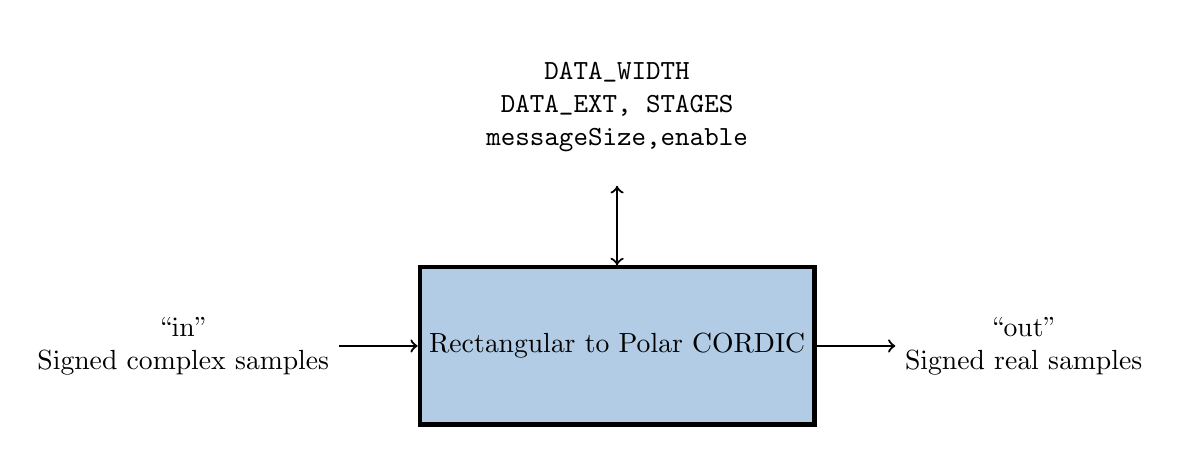
\begin{tikzpicture}[% List of styles applied to all, to override specify on a case-by-case
			every node/.style={
				align=center,  		% use this so that the "\\" for line break works
				minimum size=2cm	% creates space above and below text in rectangle
			},
			every edge/.style={draw,thick}
		]
		\node[rectangle,ultra thick,draw=black,fill=blue](R2){\Comp};
		\node[rectangle,draw=white,fill=white](R3)[left= of R2]{``in'' \\ Signed complex samples};
		\node[rectangle,draw=white,fill=white](R4)[right= of R2]{``out'' \\ Signed real samples};
		\node[rectangle,draw=white,fill=white](R5)[above= of R2]{\verb+DATA_WIDTH+ \\ \verb+DATA_EXT, STAGES+ \\ \verb+messageSize,enable+};
		\path[->]
		(R3)edge []	node [] {} (R2)
		(R2)edge []	node [] {} (R4)
		(R2)edge []	node [] {} (R5)
		(R5)edge []	node [] {} (R2)
		;
	\end{tikzpicture}
\end{center}

\subsection*{State Machine}
None

\newpage

\section*{Source Dependencies}
\subsection*{\comp.hdl}
\begin{itemize}
	\item projects/assets/components/dsp\_comps/rp\_cordic.hdl/rp\_cordic.vhd
	\item projects/assets/hdl/primitives/dsp\_prims/dsp\_prims\_pkg.vhd
	      \subitem projects/assets/hdl/primitives/dsp\_prims/cordic/src/cordic\_rp.vhd
	      \subitem projects/assets/hdl/primitives/dsp\_prims/cordic/src/cordic.vhd
	      \subitem projects/assets/hdl/primitives/dsp\_prims/cordic/src/cordic\_stage.vhd
	\item projects/assets/hdl/primitives/misc\_prims/misc\_prims\_pkg.vhd
	      \subitem projects/assets/hdl/primitives/misc\_prims/round\_conv/src/round\_conv.vhd
	\item projects/assets/hdl/primitives/util\_prims/util\_prims\_pkg.vhd
	      \subitem projects/assets/hdl/primitives/util\_prims/pd/src/peakDetect.vhd
\end{itemize}

\subsection*{\rcc_comp.rcc}
\begin{itemize}
	\item projects/assets/components/dsp\_comps/\rcc_comp.rcc/\rcc_comp.rcc
\end{itemize}

\begin{landscape}
\section*{Component Spec Properties}
	\begin{scriptsize}
		\begin{longtable}{|p{3cm}|p{1.5cm}|c|c|c|c|c|p{7cm}|}
			\hline
			\rowcolor{blue}
			Name               & Type   & SequenceLength & ArrayDimensions & Accessibility      & Valid Range & Default & Usage                                        \\
			\hline
			\verb+DATA_WIDTH+  & UChar  & -              & -               & & -           & -       & Data width of complex input and real output \\
			\hline
			\verb+DATA_EXT+    & UChar  & -              & -               & & -           & -       & Number of growth bits implemented by CORDIC  \\
			\hline
			\verb+STAGES+      & UChar  & -              & -               & & -           & -       & Number of CORDIC stages to implement          \\
			\hline
			\verb+messageSize+ & UShort & -              & -               & Writable & 8192        & 8192    & Number of bytes in output message (Not implemented by Version 2) \\
			\hline
			\verb+enable+      & Bool   & -              & -               & Writable & Standard    & true    & Enable(true) or bypass(false)                                      (Not implemented by Version 2) \\
			\hline
		\end{longtable}
	\end{scriptsize}

	\section*{Worker Properties}
	\subsection*{\comp.hdl}
	\begin{scriptsize}
		\begin{longtable}{|p{3cm}|p{2cm}|c|c|c|c|c|c|p{6cm}|}
			\hline
			\rowcolor{blue}
			Type         & Name              & Type  & SequenceLength & ArrayDimensions & Accessibility & Valid Range & Default & Usage                                                    \\
			\hline
			SpecProperty & \verb+DATA_WIDTH+ & -     & -              & -               & Parameter     & 8-16        & 16      & Real input and complex output data width                 \\
			\hline
			SpecProperty & \verb+DATA_EXT+   & -     & -              & -               & Parameter     & 6           & 6       & CORDIC requirement: Number of extension bits                 \\
			\hline
			SpecProperty & \verb+STAGES+     & -     & -              & -               & Parameter     & 8-16        & 16      & Number of CORDIC stages implemented                      \\
			\hline
			Property & \verb+PEAK_MONITOR+     & Bool     & -              & -               & Parameter     & Standard        & true      & Enable/Disable build-time inclusion of peak monitoring          \\
			\hline
			Property     & \verb+peak+  & Short & -              & -               & Volatile      & Standard    & -       & Peak value of FM Discriminator output \\
			\hline
			Property     & \verb+magnitude+  & Short & -              & -               & Volatile      & Standard    & -       & Magnitude of I/Q vector. May be useful for gain control \\
			\hline

		\end{longtable}
	\end{scriptsize}

	\subsection*{\rcc_comp.rcc}
	\begin{scriptsize}
		\begin{longtable}{|p{\dimexpr0.125\linewidth-2\tabcolsep\relax}
                  |p{\dimexpr0.1\linewidth-2\tabcolsep\relax}
                  |p{\dimexpr0.05\linewidth-2\tabcolsep\relax}
                  |p{\dimexpr0.100\linewidth-2\tabcolsep\relax}
                  |p{\dimexpr0.100\linewidth-2\tabcolsep\relax}
                  |p{\dimexpr0.1\linewidth-2\tabcolsep\relax}
                  |p{\dimexpr0.1\linewidth-2\tabcolsep\relax}
                  |p{\dimexpr0.1\linewidth-2\tabcolsep\relax}
                  |p{\dimexpr0.2\linewidth-2\tabcolsep\relax}|}
			\hline
			\rowcolor{blue}
			Type         & Name              & Type  & SequenceLength & ArrayDimensions & Accessibility & Valid Range & Default & Usage                                                    \\
			\hline
			SpecProperty & \verb+DATA_WIDTH+ & -     & -              & -               & Parameter     & 16        & 16      & Added here to be a FSK workalike, the implementation does not use this. \\
			\hline
			SpecProperty & \verb+DATA_EXT+   & -     & -              & -               & Parameter     & 6           & 6       & CORDIC requirement, the implementation does not use this. \\
			\hline
			SpecProperty & \verb+STAGES+     & -     & -              & -               & Parameter     & 8-16        & 16      & Used to truncate data to match HDL implementation \\
			\hline
			Property     & \verb+magnitude+  & Short & -              & -               & Volatile      & Standard    & -       & Magnitude of I/Q vector. May be useful for gain control \\
			\hline			
			Property & \verb+AdditionalDelay+     & UChar     & -              & -               & Parameter     & Standard        & 8      & Additional number of delays over CORDIC stages (STAGES) to match HDL implementation.          \\
			\hline
			Property     & \verb+StageDelay+  & UChar & -              & -               & Parameter      & Standard    & STAGES + AdditionalDelay       & Number of delays to match HDL implementation. \\
			\hline

		\end{longtable}
	\end{scriptsize}

	\section*{Component Ports}
	\begin{scriptsize}
		\begin{tabular}{|M{2cm}|M{1.5cm}|M{4cm}|c|c|M{9cm}|}
			\hline
			\rowcolor{blue}
			Name & Producer & Protocol           & Optional & Advanced & Usage                  \\
			\hline
			in   & false    & iqstream\_protocol & false    & -        & Signed complex samples \\
			\hline
			out  & true     & rstream\_protocol  & false    & -        & Signed real samples    \\
			\hline
		\end{tabular}
	\end{scriptsize}

	\section*{Worker Interfaces}
	\subsection*{\comp.hdl}
	\begin{scriptsize}
		\begin{tabular}{|M{2cm}|M{1.5cm}|c|c|M{12cm}|}
			\hline
			\rowcolor{blue}
			Type            & Name & DataWidth & Advanced                & Usage                  \\
			\hline
			StreamInterface & in   & 32        & - & Signed complex samples \\
			\hline
			StreamInterface & out  & 16        & InsertEOM=1 & Signed real samples    \\
			\hline
		\end{tabular}
	\end{scriptsize}
\end{landscape}

\section*{Control Timing and Signals}
The Rectangular to Polar CORDIC worker uses the clock from the Control Plane and standard Control Plane signals. This worker has a start-up transient delay of \verb+STAGES++8 valid samples. This means that once the input is ready and valid and the output is ready, it takes that many valid input samples before the first output sample is made available. The delays for this worker are itemized be as follows:
\begin{itemize}
	\item 2 : rp\_cordic.vhd
	\item 5 : rp\_cordic.vhd/cordic\_rp.vhd
	\item STAGES : rp\_cordic.vhd/cordic\_rp.vhd/cordic.vhd/cordic\_stage.vhd 
	\item 1 : cordic\_rp.vhd/round\_conv.vhd
\end{itemize}

\begin{tabular}{|M{4.5cm}|M{1cm}|M{1cm}|M{1.5cm}|M{2cm}|M{1cm}|M{1cm}|M{2.5cm}|}
	\hline
	\rowcolor{blue}
	Latency                      \\
	\hline
	\verb+STAGES++8 clock cycles \\
	\hline
\end{tabular}

\begin{landscape}
\section*{Worker Configuration Parameters}
\subsubsection*{\comp.hdl}
%\input{../../\ecomp.hdl/configurations.inc}
\section*{Performance and Resource Utilization}
\subsubsection*{\comp.hdl}
%\input{../../\ecomp.hdl/utilization.inc}
\end{landscape}
\section*{Test and Verification}
	One test case is implemented to validate the \Comp{} component:
	\begin{itemize}
		\item[1)] Normal mode
	\end{itemize}
	The input file is a waveform with a single tone at 27 Hz sampled at 10 kHz. The complex waveform is then scaled to fixed-point signed 16-bit integers, using a maximal amplitude of 32,767. Time and frequency domain plots may be viewed in Figures \ref{fig:in_time_tone} and \ref{fig:in_freq_tone} below, respectively.\par\medskip
	\begin{figure}[ht]
	\centering
	\begin{minipage}{.5\textwidth}
		\centering\includegraphics[width=1.0\linewidth]{input_time_tone}
		\captionof{figure}{Time Domain Complex Tone}
		\label{fig:in_time_tone}
	\end{minipage}%
	\begin{minipage}{.5\textwidth}
		\centering\includegraphics[width=1.0\linewidth]{input_freq_tone}
		\captionof{figure}{Frequency Domain Complex Tone}
		\label{fig:in_freq_tone}
	\end{minipage}
\end{figure}
	\noindent The output file is first checked that the data is not all zero and is then checked for the expected length. Once these quick checks are made, the complex input data is transformed into expected magnitude and phase arrays using Equations \ref{eq:1} and \ref{eq:2}. The expected phase array then implements the FM discriminator subtractor to create an array of the expected phase difference. These two expected value arrays are compared sample-by-sample with the measured phase output array from the UUT and the single value magnitude property from the UUT. Error checks are then calculated for the average peak error, the magnitude peak error, and the phase peak error. Should any of these three error values be more than one (the difference between each expected and measured value is allowed to be no greater than one) the overall test fails. Figure \ref{fig:out_time_real} depicts the conversion results of the single tone input, which shows no more than a $\pm1$ deviation from the expected result. Equation \ref{eq:4} is used to form Equation \ref{eq:5}, which validates the result shown in Figure \ref{fig:out_time_real}.

{\centering\captionsetup{type=figure}\includegraphics[scale=0.4]{output_time_real}\par\captionof{figure}{Time Domain Real Data}\label{fig:out_time_real}}

\begin{equation} \label{eq:5}
	d\phi = \frac{2f*2^{DATAWIDTH-1}}{F_s} = \frac{2*27*32,768}{10,000} = 176.9472
\end{equation}
\end{document}
